\documentclass[%
 reprint,
%superscriptaddress,
%groupedaddress,
%unsortedaddress,
%runinaddress,
%frontmatterverbose, 
%preprint,
%preprintnumbers,
%nofootinbib,
%nobibnotes,
%bibnotes,
 amsmath,amssymb,
 aps,
%pra,
%prb,
%rmp,
%prstab,
%prstper,
%floatfix,
]{revtex4-2}

\usepackage{graphicx}% Include figure files
\usepackage{dcolumn}% Align table columns on decimal point
\usepackage{bm}% bold math
\usepackage{physics}
\usepackage{cancel}
%\usepackage{hyperref}% add hypertext capabilities
%\usepackage[mathlines]{lineno}% Enable numbering of text and display math
%\linenumbers\relax % Commence numbering lines

%\usepackage[showframe,%Uncomment any one of the following lines to test 
%%scale=0.7, marginratio={1:1, 2:3}, ignoreall,% default settings
%%text={7in,10in},centering,
%%margin=1.5in,
%%total={6.5in,8.75in}, top=1.2in, left=0.9in, includefoot,
%%height=10in,a5paper,hmargin={3cm,0.8in},
%]{geometry}

\begin{document}

\preprint{APS/123-QED}

\title{MacCormack Finite Difference Solver for Ideal Magnetrohydrodynamics}% Force line breaks with \\

\author{Evan Bluhm}
%  \altaffiliation[Also at ]{Physics Department, XYZ University.}%Lines break automatically or can be forced with \\
% \author{Second Author}%
%  \email{Second.Author@institution.edu}
% \affiliation{%
%  Authors' institution and/or address\\
%  This line break forced with \textbackslash\textbackslash
% }%


\date{May 21, 2021}% It is always \today, today,
             %  but any date may be explicitly specified
\begin{abstract}

We present a Python code to solve the time-dependent, nonlinear ideal magnetohydrodynamic equations in three dimensions using a MacCormack finite difference method. We apply the model to two test problems: the Brio-Wu shock tube, and a screw pinch equilibrium.

% % \begin{description}
% % \item[Usage]
% % Secondary publications and information retrieval purposes.
% % \item[Structure]
% % You may use the \texttt{description} environment to structure your abstract;
% % use the optional argument of the \verb+\item+ command to give the category of each item. 
% % \end{description}
\end{abstract}

%\keywords{Suggested keywords}%Use showkeys class option if keyword
                              %display desired
\maketitle

%\tableofcontents


\section{Introduction}

We have previously implemented a particle-in-cell model to investigate phenomena which occur on the order of several hundred Debye lengths, or over a similar number of cycles of the plasma electron frequency. The particle model has a straightforward implementation, but modeling of full laboratory plasma configurations requires prohibitively many particles. To model phenomena at larger scales, we now move to a fluid description of the plasma.

The equations of ideal magnetohydrodynamics (MHD) capture much of the behavior of well-magnetized plasmas which have a high degree of ion collisionality and low resistivity. Using a fluid description allows us to model phenomena at much larger spatial and temporal scales.

Here, we outline the implementation of a 3-dimensional MHD solver using a MacCormack finite difference scheme to integrate the nonlinear ideal MHD equations. The solver includes additional artificial viscosity to reduce dispersive errors. The stability and accuracy of the implementation are benchmarked against a standard test of MHD solvers, the Brio-Wu shock tube test.

\section{Ideal Magnetohydrodynamics}
The equations of ideal MHD can be written in the following conservative form:
\begin{equation}
\pdv{}{t}\vec Q + \div \vec T = 0 
\end{equation}
\begin{equation}
\vec Q = [\rho, \rho v_x, \rho v_y, \rho v_z, B_x, B_y, B_z, e]
\end{equation}
\begin{equation}
\vec T = \begin{bmatrix}
\rho \vec v \\
\rho \vec v \vec v - \frac{\vec B \vec B}{\mu_0} - \left( p + \frac{B^2}{2 \mu_0} \right) \vec{1} \\
\vec v \vec B - \vec B \vec v \\
\left( e + p + \frac{B^2}{2 \mu_0} \right) \vec v - \frac{\vec B \cdot \vec v}{\mu_0} \vec B
\end{bmatrix}
\end{equation}
where $\rho$ is the plasma mass density, $\vec v$ is the center-of-mass velocity, $\vec B$ is the local magnetic field, $p$ is the plasma pressure, and $e$ is the energy density:
\begin{equation}
e = \frac{p}{\gamma - 1} + \frac{1}{2} \rho v^2 + \frac{B^2}{2 \mu_0}
\end{equation}
The ideal MHD system is a nonlinear, hyperbolic system of partial differential equations. To cast a well-posed problem, we require sufficient initial conditions and boundary conditions. The value of $\vec Q$ at all spatial locations at $t = 0$ is a sufficient initial condition. We may define different boundary conditions for different types of boundary. For a solid, conducting wall, the boundary conditions are $\vu n \cdot \vec v = 0$ and $\pdv{}{t} \vec B \cdot \vu n = 0$. We may also define periodic boundary conditions, such that $Q(x + L) = Q(x)$ for a domain $x \in [0, L]$.

\section{Finite Difference Method}

Our code attempts to numerically solve the ideal MHD equations by calculating $Q$ at discrete points in space and time, approximating the derivatives with finite difference expressions. We approximate the ideal MHD partial differential equations using the MacCormack method, which is second-order accurate in time and space. Stepping forwards in time is done in two steps. First, a predictor step uses a forward difference to estimate the value of $Q$ at time $t = (n+1)\Delta t$:
\begin{eqnarray*}
\overline{Q} _{i,j,k} ^{n+1} & = & Q_{i,j,k} ^n - \frac{\Delta t}{\Delta x} (F_{i+1, j, k}^n - F_{i, j, k} ^n) \\
& & - \frac{\Delta t}{\Delta y} (G_{i, j+1, k} ^n - G_{i, j, k} ^n) - \frac{\Delta t}{\Delta z} (H_{i, j, k+1} ^n - H_{i, j, k} ^n)
\end{eqnarray*}
where $F$, $G$, and $H$ are the fluxes in the x, y, and z directions:
\begin{equation}
\pdv{Q}{t} + \pdv{F}{x} + \pdv{G}{y} + \pdv{H}{z} = 0
\end{equation}
and $F_{i, j, k} ^n$ is the value of $F$ evaluated using the value of $Q_{i, j, k} ^n$. The corrector step is a backwards difference using the estimated value  $\overline{Q}$:
\begin{eqnarray*}
\overline{\overline{Q}} _{i,j,k} ^{n+1} & = & Q_{i,j,k} ^n - \frac{\Delta t}{\Delta x} (\overline{F}_{i, j, k}^n - \overline{F}_{i-1, j, k} ^n ) \\
& & - \frac{\Delta t}{\Delta y} (\overline{G}_{i, j, k} ^n - \overline{G}_{i, j-1, k} ^n) - \frac{\Delta t}{\Delta z} (\overline{H}_{i, j, k} ^n - \overline{H}_{i, j, k-1} ^n)
\end{eqnarray*}
Finally, we use a simple average of the predictor and corrector to obtain the value of $Q$ at time $t = (n+1) \Delta t$
\begin{equation}
Q_{i, j, k} ^{n+1} = \frac{\overline{Q}_{i, j, k} + \overline{\overline{Q}}_{i, j, k}}{2}
\end{equation}
We have implemented this MacCormack time step within the \texttt{maccormack\_time\_step()} function in the \texttt{mhd1.methods} module.

\section{MHD Finite Difference Solver}

\subsection{Initial Conditions}
We have written a Python code to solve the ideal MHD equation system using the MacCormack finite difference method, assuming solid conducting wall boundary conditions in $x$ and $y$, and periodic boundary conditions in $z$. The model takes as inputs:
\begin{itemize}
    \item The number of grid points in $x$, $y$, and $z$, and the associated length of each domain.
    \item Time step $\Delta t$ and a maximum time $t_{max}$.
    \item The initial value of $Q_{i,j,k}$ at each grid position. $Q(t=0)$ is an array of size $(8, M_x, M_y, M_z)$.
\end{itemize}
\subsection{Visualization}
Plotting methods within the \texttt{mhd1.plots} module can be used to conveniently display the initial value of $Q$ in several orthogonal projections, as shown in Figure \ref{fig:initial-conditions-plot}. The same visualization format is used to animate the evolution of the solution over time, making it easier to identify waves and instabilities.
\subsection{Boundary Conditions}
To optimize the performance of the solver's time step, a particular set of boundary conditions is ``hard-coded.'' The $z$ domain is assumed to be periodic:
\begin{equation}
Q_{i, j, 0} = Q_{i, j, M_z} \qquad Q_{i, j, M_z + 1} = Q_{i, j, 1}
\end{equation}
In the $x$ and $y$ directions, we explicitly assume solid, conducting walls. In the $x$ direction, we enforce the following at each time step:
\begin{equation}
(\rho v_x) _{0, j, k} ^n = 0 \qquad (\rho v_x) _{M_x-1, j, k} ^n = 0
\end{equation}
\begin{equation}
(B_x) _{0, j, k} ^n = (B_x) _{0, j, k} ^{0}
\end{equation}
\begin{equation}
(B_x)_{M_x-1, j, k} ^n = (B_x) _{M_x-1, j, k} ^{0}
\end{equation}
where indexes $i$ and $n$ start at 0. A similar set of conditions holds at the edges of the $y$ domain.
\subsection{Artificial Diffusion}

Finite difference approximations to hyperbolic partial differential equations can be prone to large oscillatory errors in the vicinity of steep gradients or discontinuities. The spatial average performed when combining the predictor and corrector steps has a diffusive effect on the solution, helping to smooth out oscillatory errors. In some cases, such as the Brio-Wu shock test described below, this is insufficient to maintain stability, and additional artificial diffusion is required. Our code contains a flag called \texttt{diffusion\_method} which determines whether to add an artificial viscosity term, so that instead we solve the following modified system of equations:
\begin{equation}
\pdv{Q}{t} + \pdv{F}{x} + \pdv{G}{y} + \pdv{H}{z} = \sigma \nabla ^2 Q
\end{equation}
If additional diffusion is turned on, our code adds a second-order centered finite difference for the diffusive term, after the predictor-corrector step:
\begin{eqnarray*}
Q_{ijk} ^{n+1} = Q_{ijk} ^{n+1} + \sigma \Delta t &  & \left[\frac{Q_{i+1, j, k} ^{n+1} - 2 Q_{i, j, k} ^{n+1} + Q_{i-1,j,k} ^{n+1}}{\Delta x^2} \right. \\
& & + \frac{Q_{i, j+1, k} ^{n+1} - 2 Q_{i, j, k} ^{n+1} + Q_{i,j-1,k} ^{n+1}}{\Delta y ^2} \\
& & \left. + \frac{Q_{i, j, k + 1} ^{n+1} - 2 Q_{i, j, k} ^{n+1} + Q_{i,j,k + 1} ^{n+1}}{\Delta z^2} \right]
\end{eqnarray*}
where the viscosity $\sigma$ is a configurable parameter. By default, it is everywhere set to a constant value of $\sigma = 0.1 \frac{\Delta x ^2}{\Delta t}$.

\begin{figure}
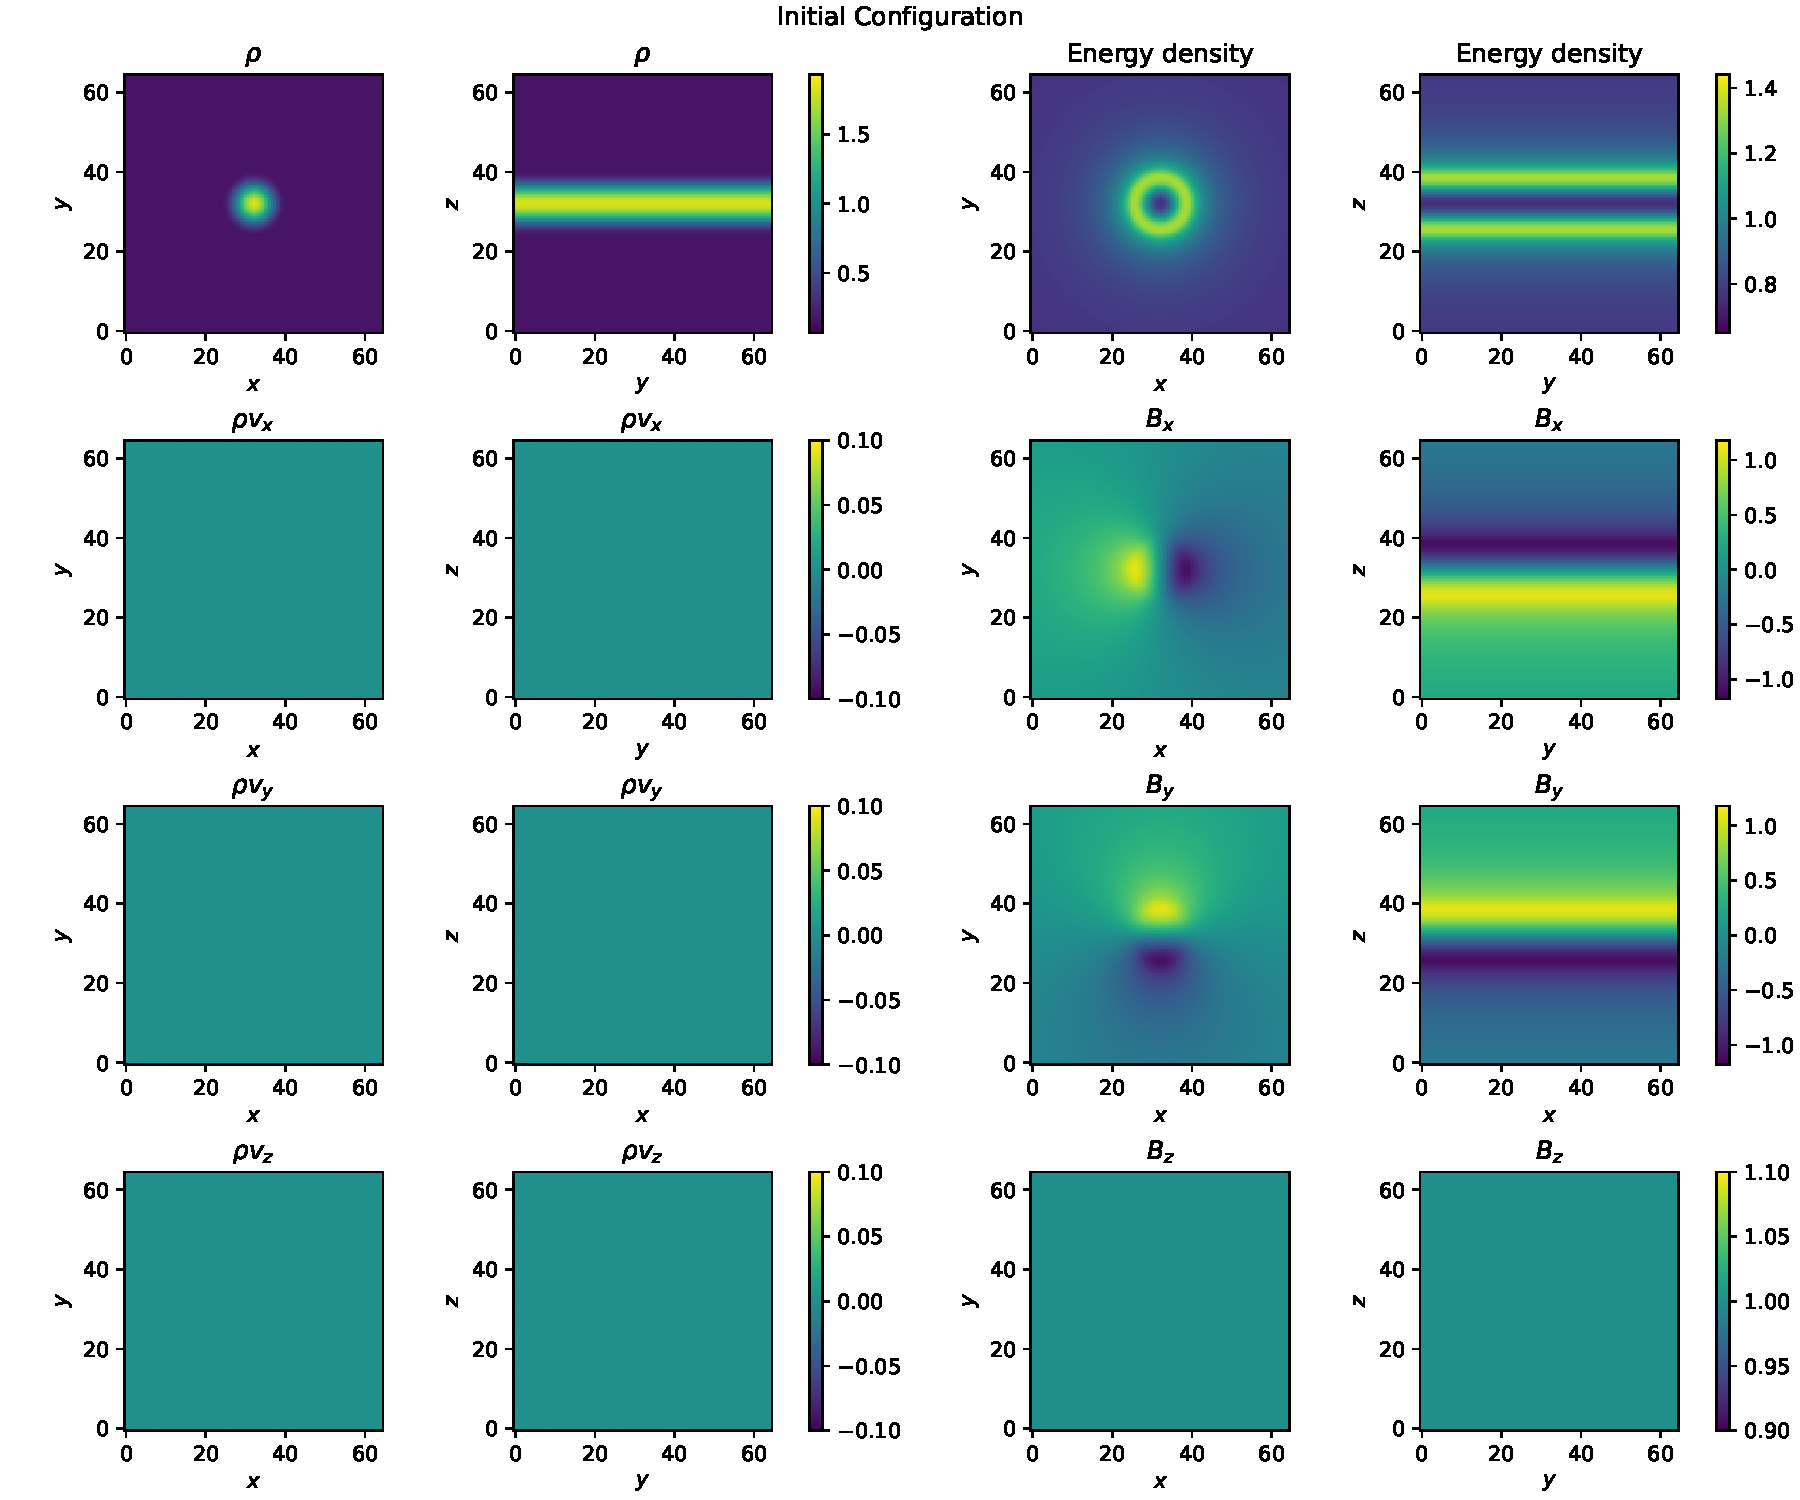
\includegraphics[width=0.9\linewidth]{proj2-2/initial_configuration.pdf}
\caption{\label{fig:initial-conditions-plot}Plot of initial conditions for a screw pinch with radius $R=8$, parabolic axial current density $j_z = 0.5(1 - r^2/R^2)$, and static axial field $B_z = 1$. Quantities shown in the x-y plane are drawn at the midpoint of the z-domain; the same is true of quantities plotted in the x-z and y-z planes. The initial pressure and magnetic field profiles are the same as those outlined in Appendix A.}
\end{figure}

\subsection{Stability}
Since the ideal MHD equations are hyperbolic, they support both forward and backward-propagating waves, with characteristics given by the sound speed, the Alfvén speed, and the slow and fast magnetosonic wave speeds. By incorporating both forward and backward differences, the MacCormack scheme is stable to waves propagating in both directions as long as the CFL condition is satisfied for waves with speed $a$:
\begin{equation}
C = \frac{a \Delta t}{\Delta x} < 1
\end{equation}
The fastest-moving wave in ideal MHD is the fast magnetosonic wave. In the x-direction, the fast magnetosonic wave travels at:
\begin{equation}
|v_{fast, x}| = |v_x| + \sqrt{\frac{1}{2}\left(a^2 + c_s ^2 - \sqrt{(a^2 + c_s ^2)^2 - 4 a_x ^2 c_s ^2} \right) }
\end{equation}
where the Alfvén wave speed is
\begin{equation}
a^2 = \frac{B^2}{\rho \mu_0} \qquad a_x ^2 = \frac{B_x ^2}{\rho \mu_0}
\end{equation}
and the sound speed is
\begin{equation}
c_s ^2 = \frac{\gamma p}{\rho}
\end{equation}
At each time step, our finite difference solver computes the Courant number at each spatial position based on the maximum possible characteristic in each direction. If the CFL stability condition is violated at any point, in any direction, the solver exits with an appropriate message.

The solution variables $\rho$ and $e$ must be positive definite at all points. We require $\rho > 0$ everywhere, since the wave characteristics become infinite as $\rho \rightarrow 0$. In the absence of oscillatory errors and dispersive effects, the ideal MHD equations automatically satisfy these conditions . However, errors introduced by our numerical model can 

\section{Data Format}

The current state $Q_{ijk} ^n$ is internally stored as an array of shape $(8, M_x, M_y, M_z)$. As we evolve the solution over time, we update the current solution in-place at the end of each time step, replacing the previous value. Several other quantities of interest are calculated at each time step and stored as timeseries values for later analysis and plotting:
\begin{itemize}
\item The total kinetic energy $KE = \int \frac{\rho v^2}{2} \dd V$
\item The total energy stored in the magnetic field $FE = \int \frac{B^2}{2 \mu_0} \dd V$
\item The total energy $TE = \sum_{ijk} e_{ijk} \Delta x \Delta y \Delta z$
\item The maximum value of $\div \vec B$ across all points in the spatial domain. While the exact MHD equations will preserve an initially divergence-free magnetic field, numerical errors will contribute to a finite divergence. Tracking the growth of $\div \vec B$ allows us to measure the size of these errors, and refine the grid spacing if needed.
\end{itemize}

Simulations may require a very small $\Delta t$ to achieve CFL stability. These runs can take a long time to complete, and maintaining the history of $Q_{ijk}$ in working memory at each time step for later plotting and analysis quickly exceeds the memory limits of most personal computers. To overcome this, our code uses the \texttt{PyTables} library to periodically write out the current state to the hard disk in the HDF5 file format. This library allows us to write data to disk in a chunked, compressed format with fast disk write performance.

On many systems, hard disk space is also a limited quantity. For longer simulations with large spatial grids, it may not be desirable to store the full solution at every time step. A \texttt{max\_history\_steps} parameter allows the user to specify the maximum number of time steps which are written out to disk. If this is smaller than $t_{max} / \Delta t$, data is only written to disk at appropriately sub-sampled time steps.

\section{Test Problems}
\begin{figure}
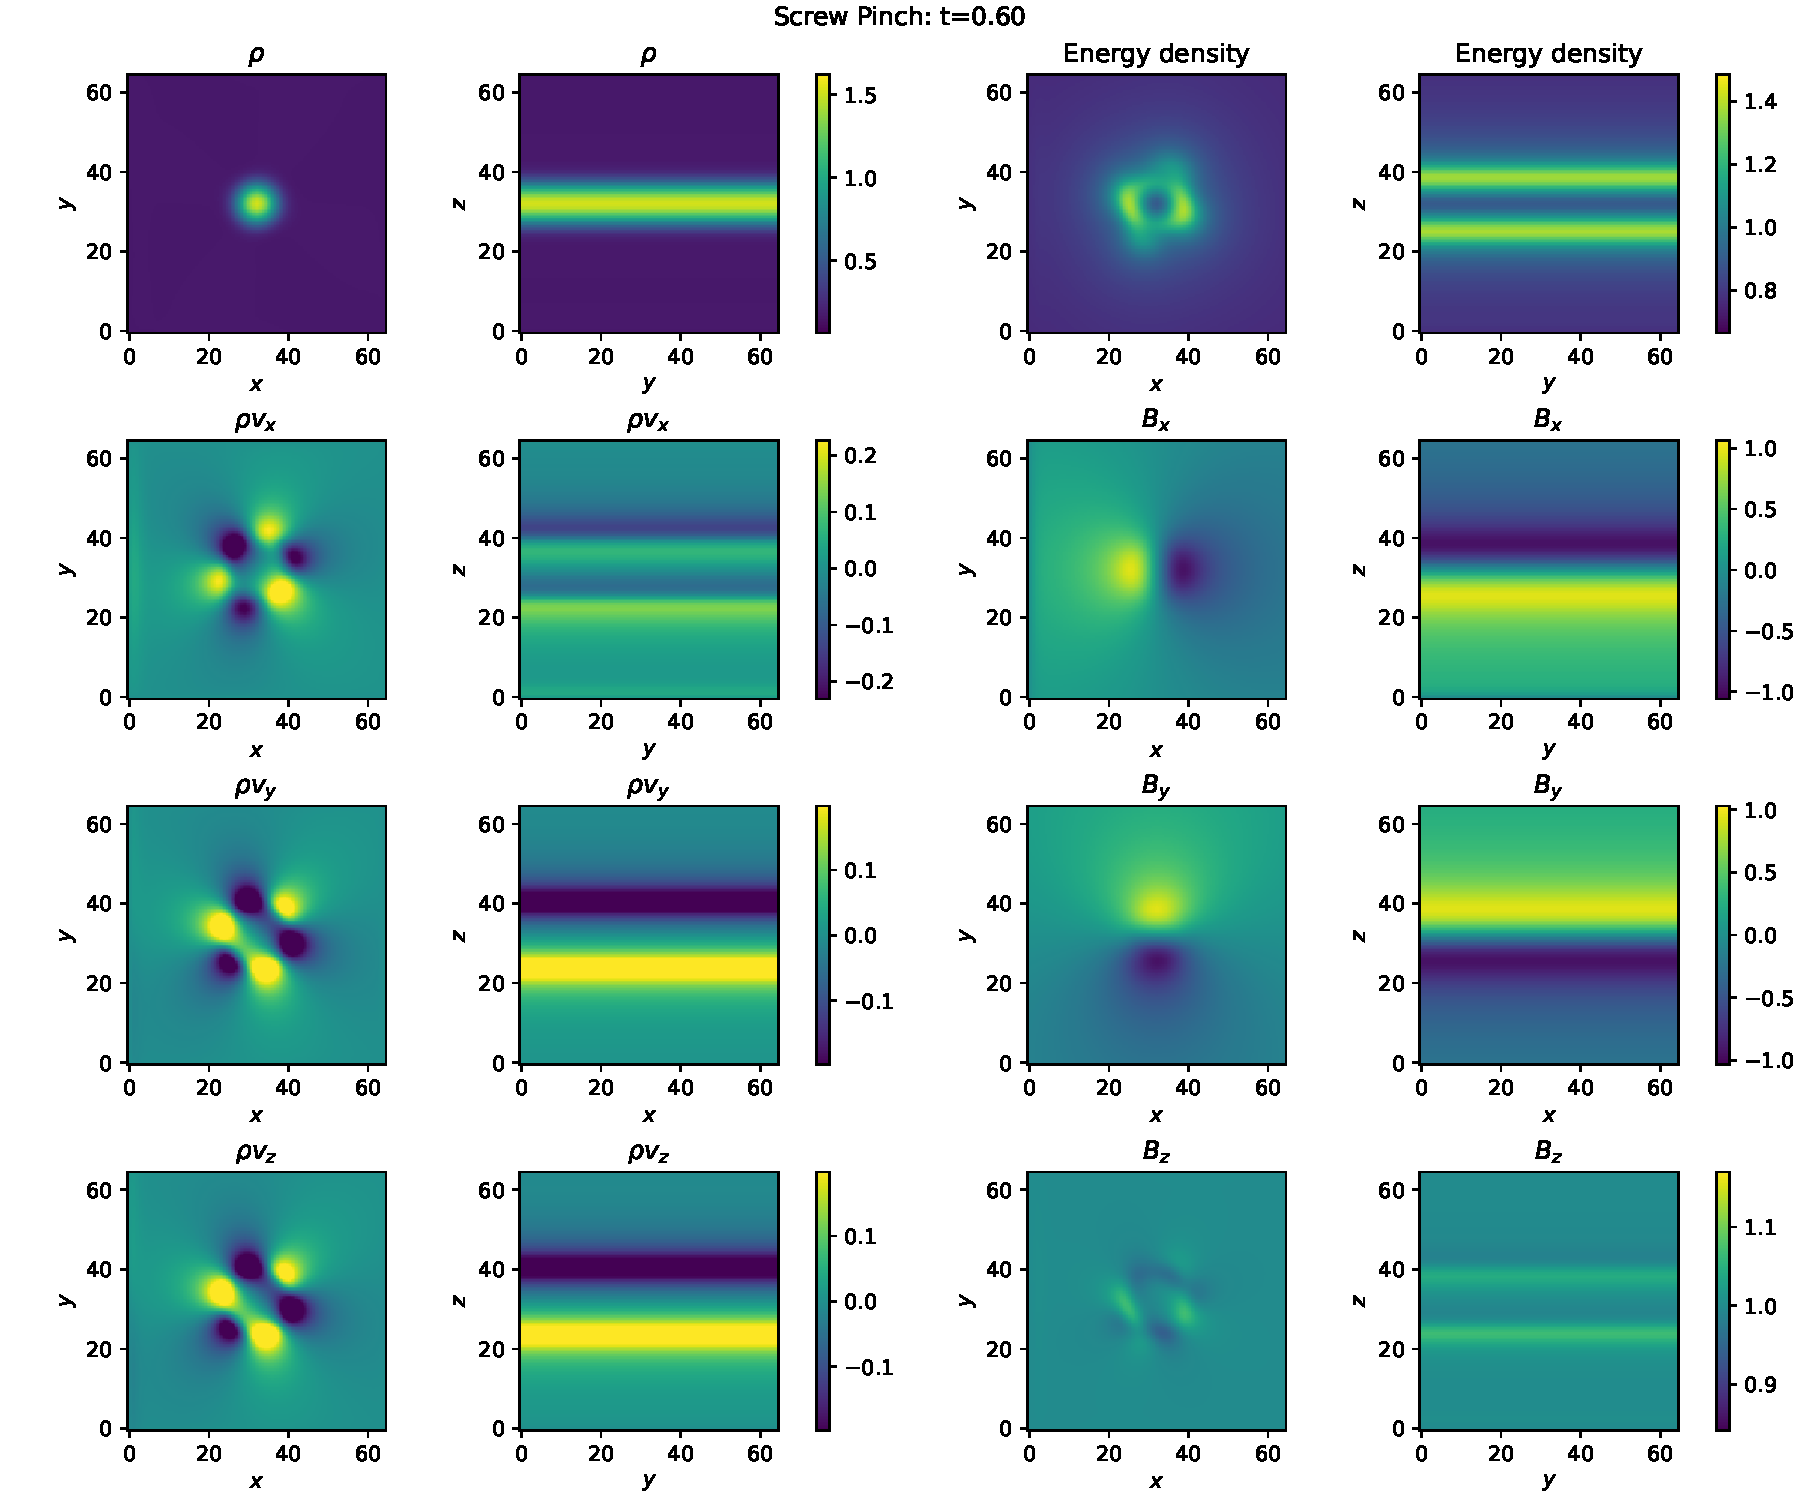
\includegraphics[width=0.9\linewidth]{proj2-2/mhd_snapshot_n_3.pdf}
\caption{\label{fig:screw-pinch-snapshot}Snapshot of the solution for the initial conditions shown in Figure \ref{fig:initial-conditions-plot} after 12 time steps with $\Delta t = 0.05$. There is no initial perturbation in the velocity. The configuration should be stable over time, but instead we see the appearance of a strong rotational mode about the pinch axis, which quickly tears the configuration apart.}
\end{figure}

\begin{figure}
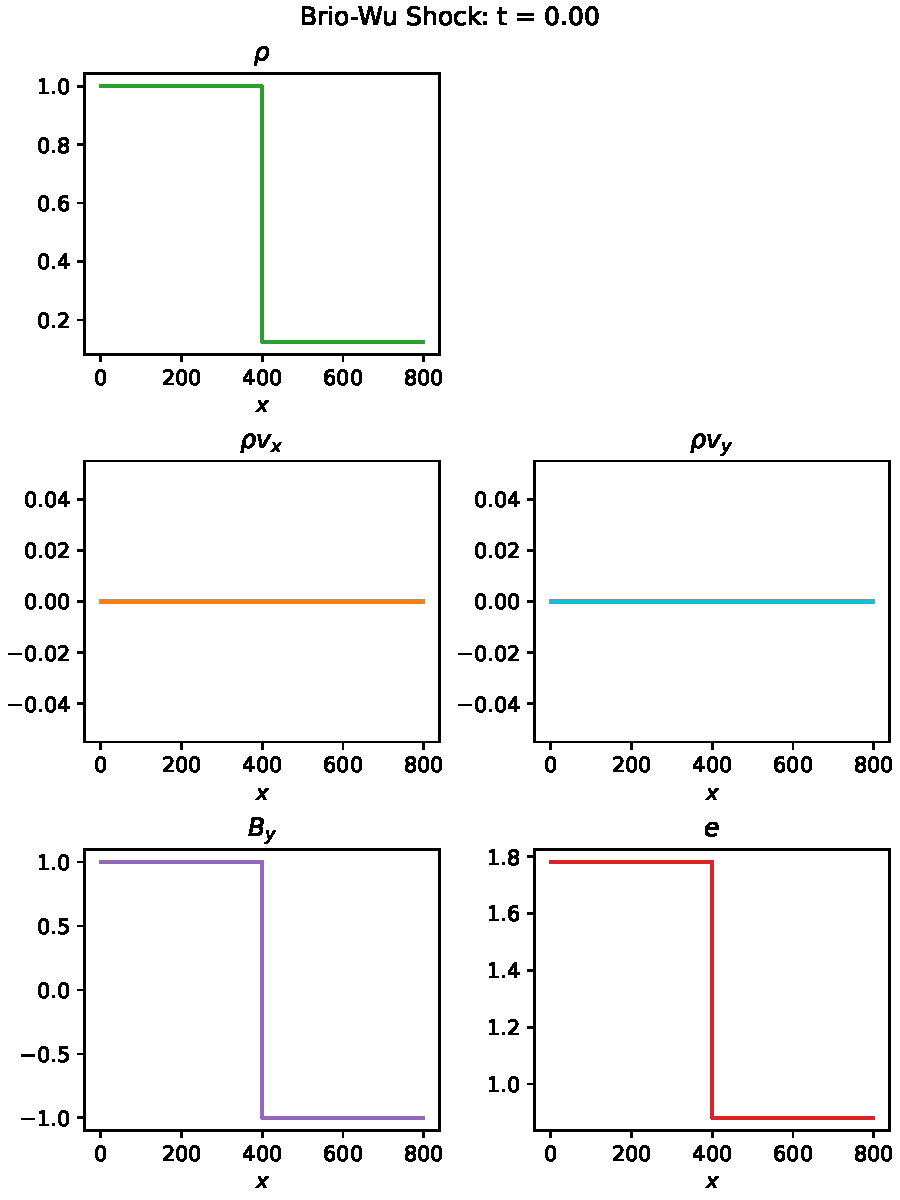
\includegraphics[width=0.7\linewidth]{proj2-2/shock_snapshots_n_0.pdf}
\caption{\label{fig:brio-wu-initial-conditions}The initial conditions for the Brio-Wu shock problem are shown at $t=0$ for $M_x = 800$, $M_y = 1$, $M_z = 1$.}
\end{figure}

\begin{figure}
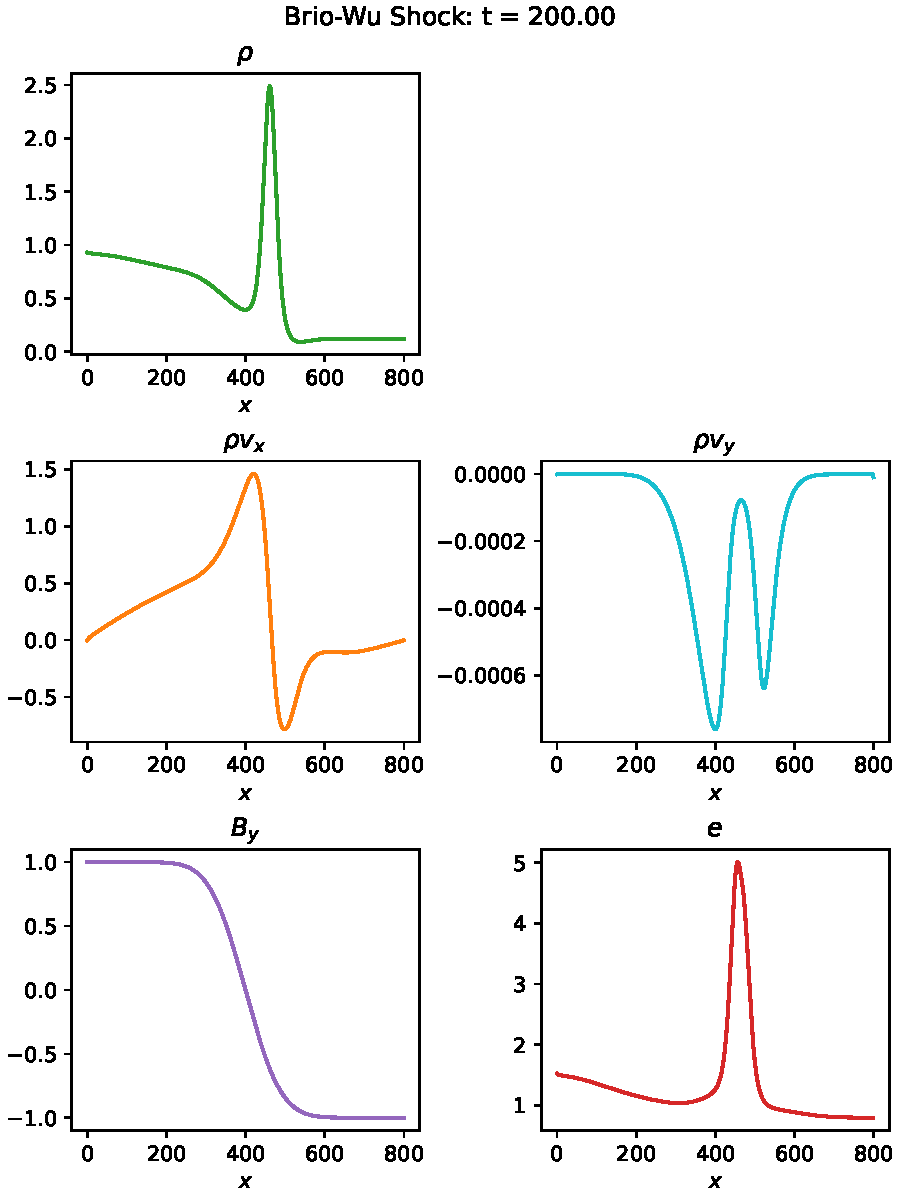
\includegraphics[width=0.7\linewidth]{proj2-2/shock_snapshots_n_20.pdf}
\caption{\label{fig:brio-wu-snapshot}Snapshot of our solver's solution to the 1-dimensional Brio-Wu shock problem. The solution from our MHD solver is shown after evolving to $t=200$ with artificial viscosity turned on. Non-physical dispersive errors have generated a density spike near $x=440$.}
\end{figure}


\subsection{Brio-Wu MHD Shock Tube Test}

As first shown in Ref. \cite{BRIO1988400}, an extension of the hydrodynamic Sod shock tube to the realm of magnetohydrodynamics is a useful test problem for MHD codes. The Brio-Wu shock tube test is posed as a 1.5D Riemann problem, with a discontinuity in the middle of the domain. The configuration generates two fast rarefaction waves, a slow compound wave, a contact discontinuity, and a slow shock wave, making it a demanding test of the wave properties of a MHD solver.
The initial condition for the shock tube is a piece-wise configuration composed of a left and right state. On the left half of the spatial domain, $\rho_l = 1$, $p_l = 1$, and $(B_y)_l = 1$. All other conserved quantities are zero:
\begin{equation}
Q_l = [1, 0, 0, 0, 0, 1, 0, 1.5] \quad x < 0
\end{equation}
The right state is $\rho_r = 0.125$, $p_r = 0.1$, $(B_y)_r = -1$:
\begin{equation}
Q_r = [0.125, 0, 0, 0, 0, -1, 0, 0.6] \quad x \geq 0
\end{equation}
These initial conditions are shown in Figure \ref{fig:brio-wu-initial-conditions}. For a grid spacing such that $\Delta x = 1$ and $\Delta t = 0.2$, this set of initial conditions gives a Courant number of $\sim 0.8$. While the CFL condition for stability is satisfied, it is not a sufficient condition to guarantee stability.

Our model's solution for the Brio-Wu shock problem is shown in Figure \ref{fig:brio-wu-snapshot}. The simulation was first performed without additional diffusion, but Gibbs phenomenon at the discontinuity generated negative densities within a few time steps, and the simulation was terminated early by the physicality checks. The solution shown in Figure \ref{fig:brio-wu-snapshot} was performed with the default artificial diffusive term. The forward and backward fast rarefaction waves are easily identifiable in the animated solution, as they are the first to travel away from the discontinuity. However, these waves are not captured in $B_y$. Worse yet, dispersive errors have generated a non-physical spike in the density which grows over time. We were not able to resolve the instability by increasing the artificial viscosity, indicating more fundamental errors in the finite difference solver.

\subsection{Screw Pinch Equilibrium}

In Appendix A, we solve for the initial conditions $Q(t=0)$ of a stationary screw pinch with a parabolic axial current and constant axial magnetic field. The initial conditions are shown in Figure \ref{fig:initial-conditions-plot}. The evolution of the solution is shown in Figure \ref{fig:screw-pinch-snapshot}, with $\Delta t=0.05$ and artificial diffusion turned on. Whereas we expect the equilibrium to remain stationary, we see the rapid growth of an axisymmetric rotational mode which quickly disrupts the configuration.

Given this unexpected result, together with the growth of non-physical modes in the Brio-Wu shock test, we conclude that our finite difference approximation to the ideal MHD equations contains outstanding implementation errors. These should be addressed before the model can be used to validate the stability conditions for equilibrium configurations.

\nocite{*}

\bibliography{proj2-2}% Produces the bibliography via BibTeX.


\onecolumngrid

\pagebreak

\appendix

\section{Screw Pinch Initial Conditions}

To provide sufficient initial conditions for the MHD system of equations, we must specify the initial value of all conserved variables ($\rho$, $\rho v_x$, $\rho v_y$, $\rho v_z$, $B_x$, $B_y$, $B_z$, $e$) at all points in the domain, and we must do so consistently with the governing equations. In this study, we wish to initialize a screw pinch in steady-state equilibrium, with a parabolic current profile of radius $R$ and constant axial magnetic field:

\begin{equation}
j _z(r, \theta, z) = \begin{cases} j_0(1 - r^2/R^2 ) \quad & \text{if} \quad r \leq R \\
0 \quad  &\text{if} \quad r > R
\end{cases}
\end{equation}
\begin{equation}
j_x = j_y = 0
\end{equation}
\begin{equation}
B_z(r, \theta, z) = {B_z}_0
\end{equation}
We must specify $B_x$ and $B_y$ consistent with Ampere's law:
\begin{equation}
\oint \vec B_\theta \cdot \dd \vec l = \mu_0 \int \vec j \cdot \dd \vec A
\end{equation}
For $r \leq R$:
\begin{eqnarray}
2 \pi r B_\theta & = & \mu_0 \int _0 ^r 2 \pi r' j_z \dd r' \\
B_\theta & = & \frac{\mu_0}{2 \pi r} \int_0 ^r 2 \pi r' j_0 \left( 1 - \frac{{r'}^2}{R^2} \right) \dd r' \\
B_\theta & = & \frac{\mu_0 j_0}{2} \left( r - \frac{r^3}{2 R^2} \right) \qquad r \leq R
\end{eqnarray}
And for $r > R$:
\begin{eqnarray}
2 \pi r B_\theta & = & \mu_0 \int _0 ^R 2 \pi r' j_z \dd r' \\
B_\theta & = & \frac{\mu_0 j_0 R^2}{4 r} \qquad r > R
\end{eqnarray}
Together,
\begin{equation}
 B_\theta = \begin{cases}\frac{\mu_0 j_0 R^2}{4 r} & \qquad r > R \\ \frac{\mu_0 j_0}{2} \left( r - \frac{r^3}{2 R^2} \right) & \qquad r \leq R \end{cases}   
\end{equation}
Converting back to Cartesian coordinates, $B_x$ and $B_y$ are given by:
\begin{equation}
B_x = - B_\theta \sin \theta \qquad B_y = B_\theta \cos \theta \qquad \tan \theta = \frac{y}{x}
\end{equation}

We can determine the initial pressure profile from $B_\theta$ and $B_z$, according to the equilibrium ideal MHD force balance condition:
\begin{equation}
\pdv{}{r} \left( p + \frac{B_\theta ^2 + B_z ^2}{2 \mu_0} \right) + \frac{B_\theta ^2}{\mu_0 r} = 0
\end{equation}
For $r \leq R$, the pressure profile must be:
\begin{eqnarray}
0 & = & \pdv{}{r} \left( p + \frac{B_\theta ^2 + B_z ^2}{2 \mu_0} \right) + \frac{B_\theta ^2}{\mu_0 r} \\
\pdv{p}{r} & = & - \frac{B_\theta ^2}{\mu_0 r} - \pdv{}{r} \left( \frac{B_z ^2 + B_\theta ^2}{2 \mu_0} \right ) \\
 & = & - \frac{j_0 ^2 \mu_0}{16 R^4}r (r^2 - 2R^2)^2 - \frac{j_0 ^2 \mu_0}{16 R^4} (3 r^5 - 8R^2 r^3 + 4 R^4 r) \\
p & = & p_0 - \frac{j_0 ^2 \mu_0}{48 R^4} (2 r^6 - 9 R^2 r^4 + 12 R^4 r^2)
\end{eqnarray}

For $r > R$, the pressure is constant:
\begin{eqnarray}
0 & = & \pdv{}{r} \left( p + \frac{B_\theta ^2 + B_z ^2}{2 \mu_0} \right) + \frac{B_\theta ^2}{\mu_0 r} \\
\pdv{p}{r} & = & - \frac{B_\theta ^2}{\mu_0 r} - \pdv{}{r} \left( \frac{B_z ^2 + B_\theta ^2}{2 \mu_0} \right ) \\
& = & - \frac{B_\theta ^2}{\mu_0 r} - \pdv{}{r} \left( \frac{1}{2 \mu_0} \left(\frac{\mu_0 j_0 R^2}{4 r} \right)^2 \right) \\
& = & - \frac{j_0 ^2 R^4}{16 \mu_0 r^3} + \frac{j_0 ^2 R^4}{16 \mu_0 r^3} \\
& = & 0
\end{eqnarray}
So the initial equilibrium pressure profile is:
\begin{equation}
p = \begin{cases} p_0 - \frac{j_0 ^2 \mu_0}{48 R^4} (2 r^6 - 9 R^2 r^4 + 12 R^4 r^2) & \quad r \leq R \\ p_0 & \quad r > R\end{cases}
\end{equation}

For a stationary equilibrium, we set $\vec v = 0$. To set an appropriate density profile $\rho(r)$, we assume that the initial distribution is isothermal, so that:
\begin{equation}
p = \rho k T_i / m_i
\end{equation}


\end{document}
